\section{The mesh}
\label{sec-mesh}

The scattered wave returned to the user is represented by its
values on a user-specified mesh, which we show here.
The mesh in the radial direction is specified piecewise, with
a half Chebyshev mesh on the inner disk (to avoid redundant density
at the center) and a normal Chebyshev mesh on other annular regions
(if any). 

\begin{figure}[h]
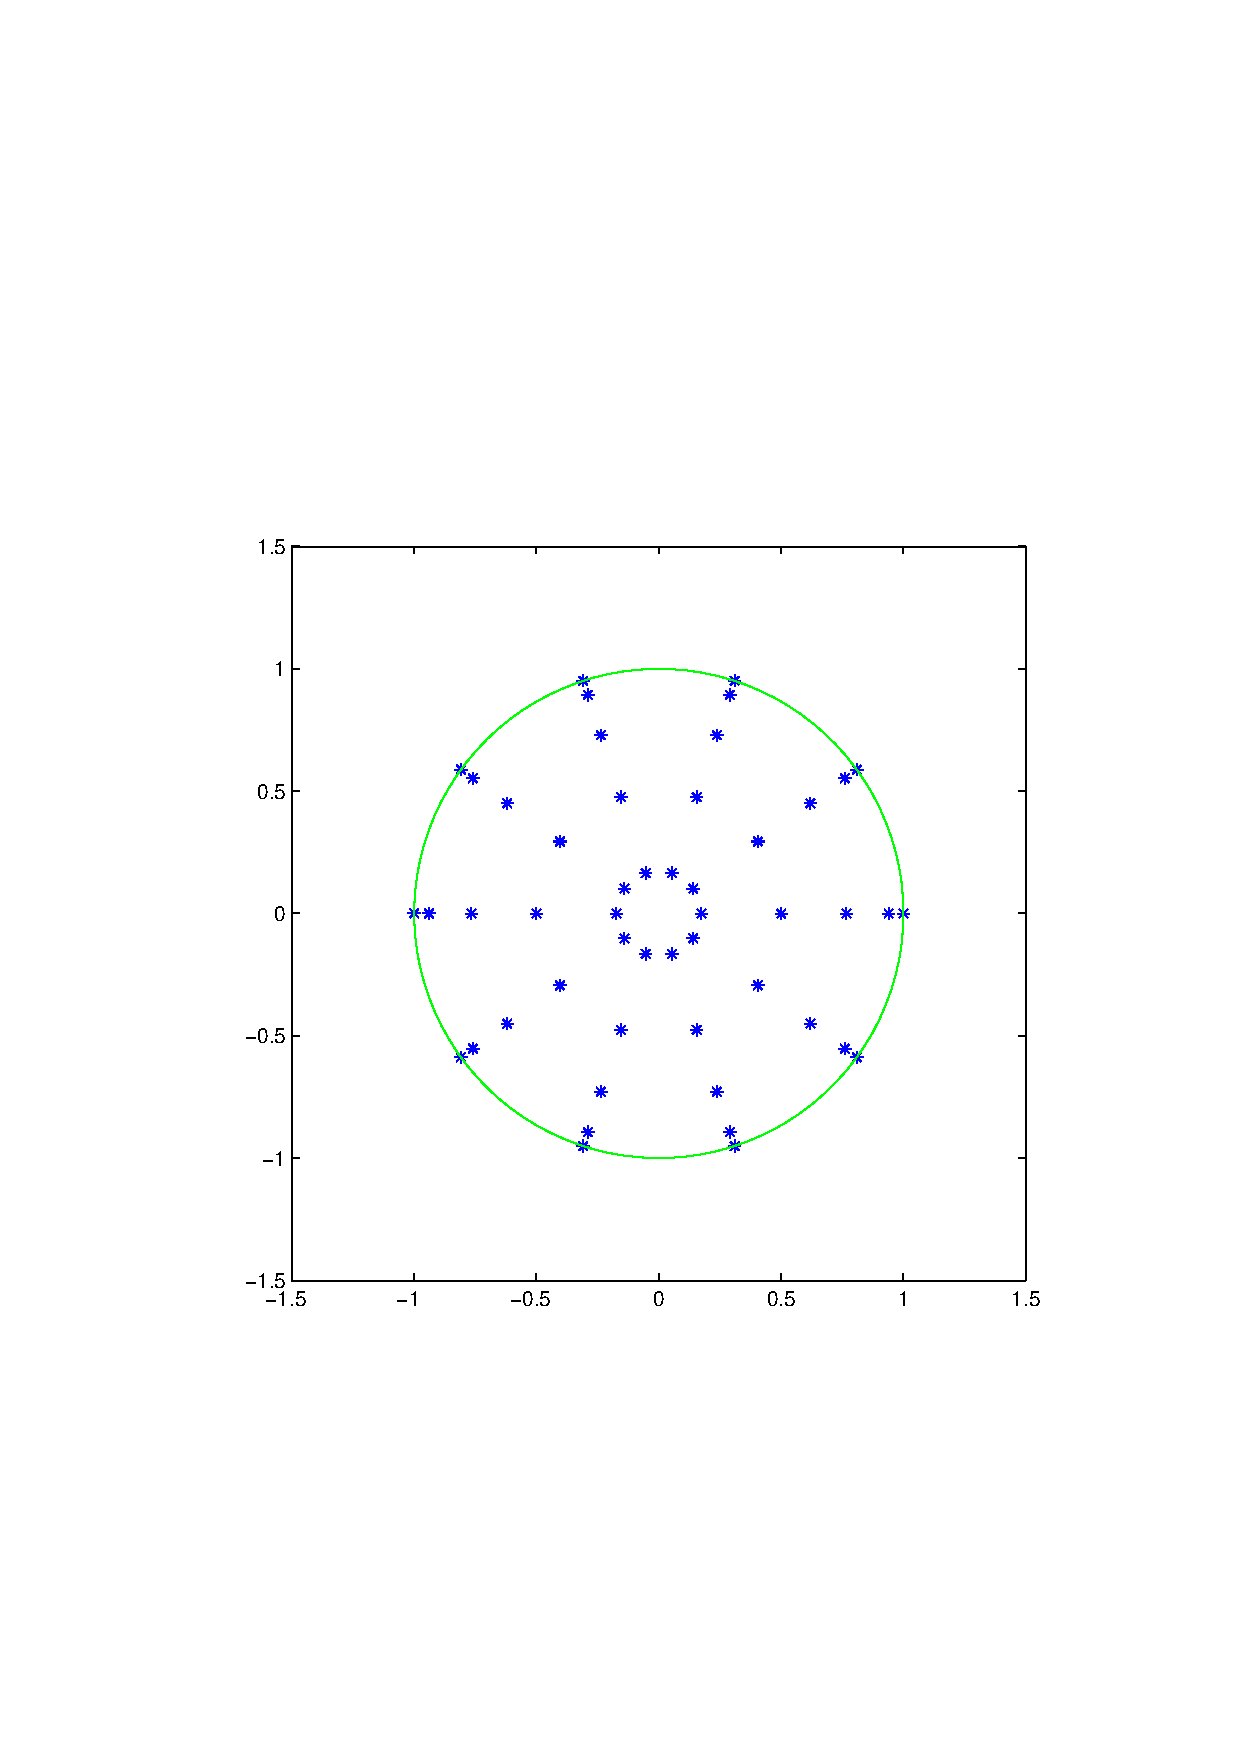
\includegraphics[width=0.49\linewidth]{figures/simplemesh.pdf}
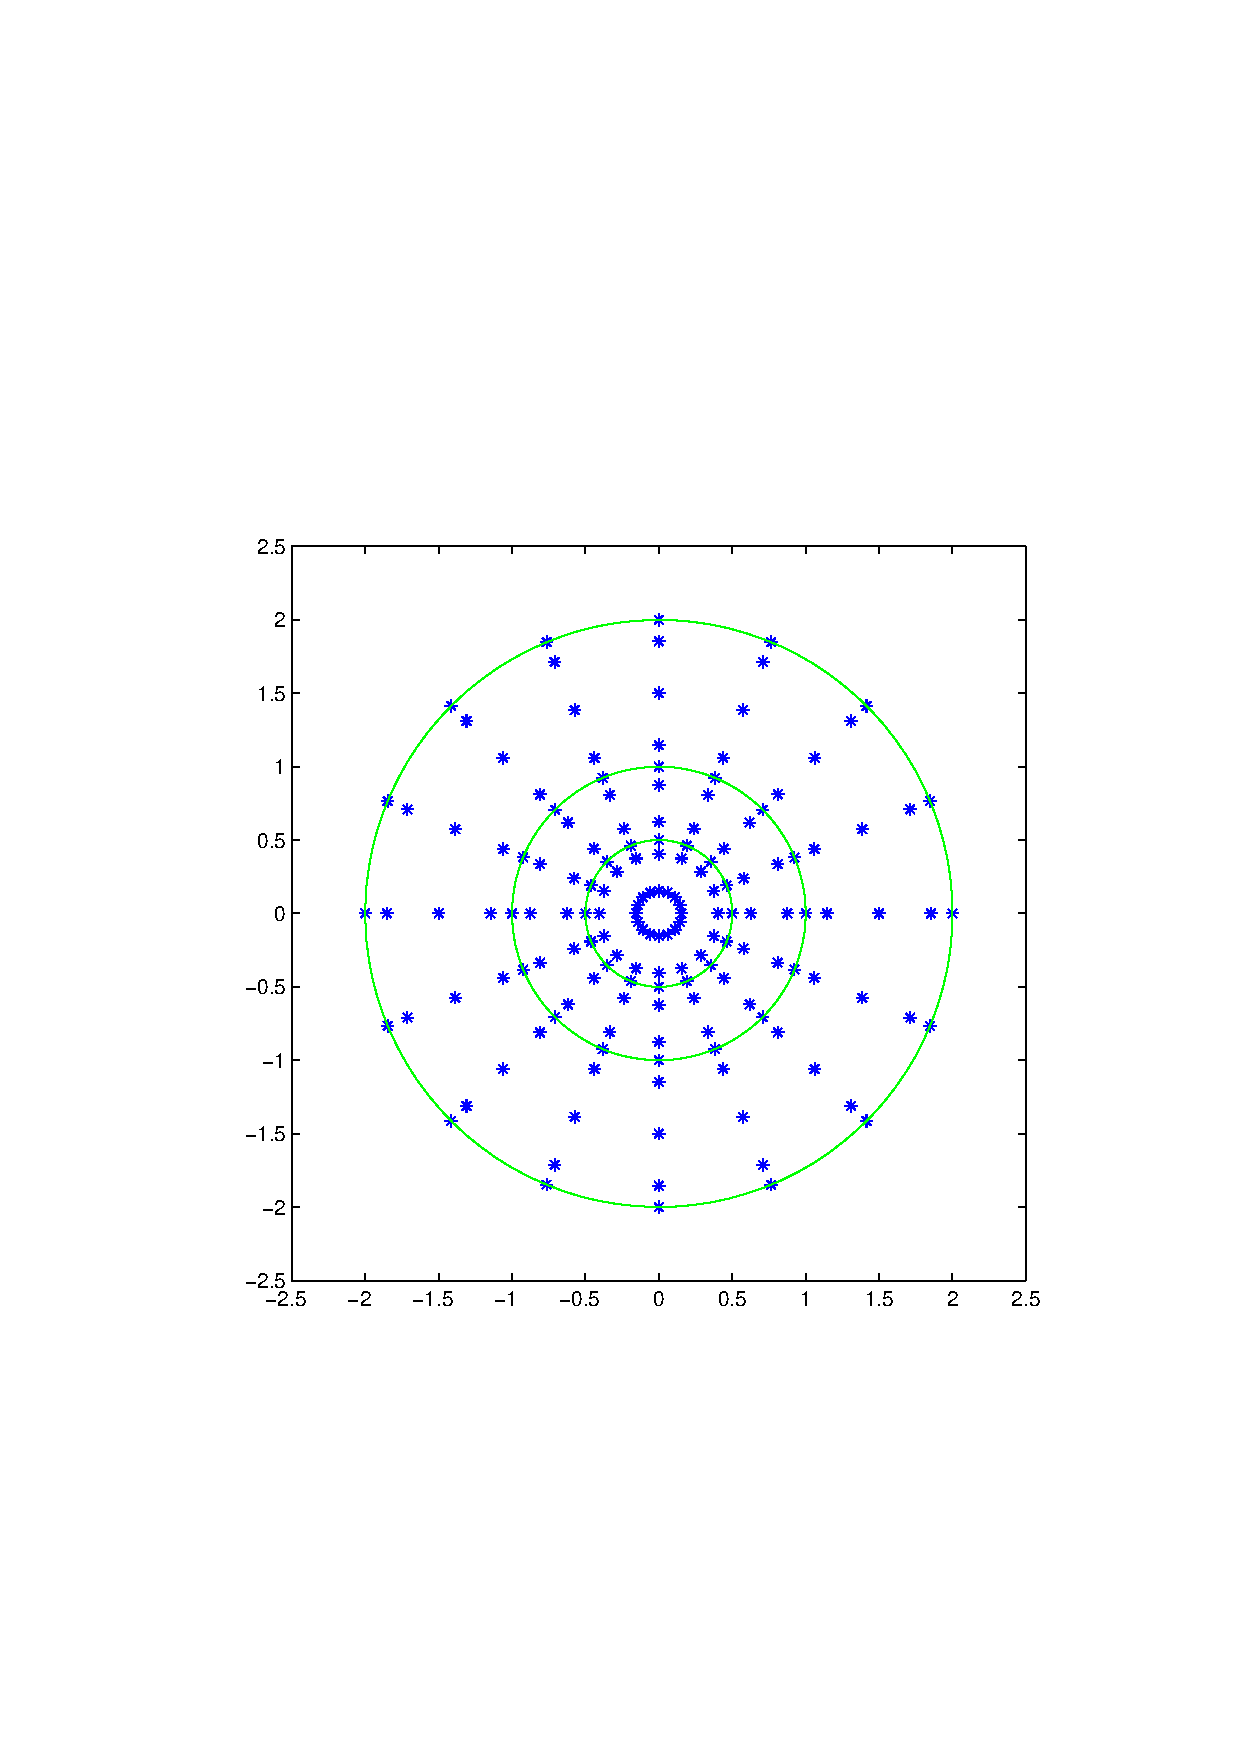
\includegraphics[width=0.49\linewidth]{figures/complicatedmesh.pdf}
\caption{Left: $R = 1$, eight $\theta$ mesh points ($N_t = 10$), 
               five points in half-Chebyshev mesh in radial 
               direction ($N_r = 5$).
         Right: Mesh specified piecewise, separately on
               $0 \le r \le 0.5$, $0.5 \le r \le 1$, and
               $1 \le r \le 2$.}
\end{figure}


